\section{Einleitung}

Der heutige Netzwerkverkehr fast tausendfach größer als vor 20 Jahre \citep{Roser_I}. Das Internet wird heutzutage für fast alle unseren alltäglichen Tätigkeiten verwendet: Soziale Netzwerke, Video und Audio-Streaming, Einkauf, behördliche Angelegenheiten und viele andere. So viel Verkehr generiert eine unermessliche Menge von Daten, die alle möglichen Inhalte beinhalten, von unschuldigen Anfragen nach einem eigenen Kontostand bis zur Ausführung von beabsichtigten Anfragen, um Systeme lahmzumachen. Um das Erste vom Zweiten zu unterscheiden, verwenden viele Firmen das sogenannte \glsfirst*{SIEM} oder die Log-Analyse-Tools. 

Das \glsfirst{NIST} definiert \gls{SIEM} als Software für die Sammlung, Anpassung, Analyse, Überwachung und Bedrohungserkennung von Sicherheitsdaten aus verschiedenen Quellen, damit das zuständige \glsfirst{SOC}  Maßnahmen ergreifen kann \citep{NIST_Definitions}. Die Bewertung dieser Daten spielt eine wesentliche Rolle bei solchen Anwendungen, da es entscheidend ist zu wissen, ob es sich um normale Anfrage oder um \glsplural{Cyberangriff} handelt. Log Analysis und Log Management beziehen sich auf die Sammlung, Bearbeitung, Speicherung und/oder Löschen, Weiterleitung und Überwachung von Loginformationen. In dieser Arbeit benutzen wir den Begriff \quotes{Log-Analyse-Tools}, um diese Systeme zu referenzieren.

In diesem Projekt recherchieren und vergleichen wir existierende \gls{SIEM} und Log-Analyse-Tools. Danach entscheiden wir uns für eine \gls{opensource} Lösung. Mit dem ausgewählten Tool wollen wir spezifische Logdateien analysieren und bewerten, damit wir demnächst potenzielle Angriffe erkennen können. Die Angriffserkennung soll automatisch mit der Eingabe von vordefinierten Regeln der \gls{mitre} Matrix stattfinden. 

\newpage
Unser Ziel ist, eine umfangreiche \gls{opensource} Lösung zu finden bzw. gesltaten, die uns ermöglichen, \glsplural{Cyberangriff} schnell und einfach zu detektieren. \gls{Proprietary} Lösungen gibt es viele auf dem Markt. Sie kosten meisten sehr viel und verlangen spezielle Kenntnis für die Verwaltung. Da solche Lösungen eher an großen Unternehmen eingeschränkt sind, beschäftigen wir uns mit dem Aufbau und Strukturierung eine eigene Lösung mithilfe von \gls{opensource} Tools. 

Diese Arbeit wird in folgende Teile geteilt: 

% OSSIN: https://sourceforge.net/projects/os-sim/
% Preludes: https://www.prelude-siem.org/projects/prelude/wiki/ManualUser
% ELK Stack

% Grafana / Promtail: https://grafana.com/products/enterprise/
%https://grafana.com/logs/% 

%https://www.ossec.net/         https://github.com/ossec/ossec-rules

% was machen sie konkrent? / Vergleich zwischen OpenSource/Proprietary/

{\setstretch{1.5}
\begin{itemize}[noitemsep]
   \item	Definition von SIEMs und Log-Analyse-Tools 
   \item	Beschreibung von existierenden Proprietary und Open Source Lösungen 
   \item	Entscheidung für die Implementation einer Open Source Lösungen 
   \item	Installation und Konfiguration von der ausgewählten Anwendung 
   \item	Definition von zwei spezifischen Cyberangriffen 
   \item	Festlegung von Regeln oder Use Cases für die automatische Erkennung von der vorherigen definierten Angriffen anhand der \gls{mitre} Matrix 
   \item	Empfang, Bearbeitung und Eingabe in der ausgewählten Lösung der spezifischen Logdateien der Hochschule 
\end{itemize}
}

\subsection{Problemstellung}
Während der Entwicklung dieser Arbeit wollen wir uns mit folgenden Fragen beschäftigen: 

{\setstretch{1.5}
% Regeln anhand mittre, automatisieren
\begin{itemize}[noitemsep]
   \item Wie können wir ein Log-Analyse-Tool so konfigurieren, dass es vordefinierten Angriffe nach der \gls{mitre} Matrix automatisch erkennen kann? 
   \item Wie können wir eine allgemeine \glsplural{usecases} definieren, sodass wir sie später für verschiedene Angriffsmuster nach \gls{mitre} Matrix leicht anpassen können?
\end{itemize}
}

\newpage
\subsection{Vorgehensweise}
Um diese oben genannten Ziele zu erreichen, verwenden wir folgenden Methoden: 

{\setstretch{1.5}
\begin{itemize}[noitemsep]
   \item	Recherche in der Fachliteratur über SIEMs und Log-Analyse-Tools Lösungen 
   \item	Vergleich zwischen verschiedenen Open Source und Proprietary Lösungen 
   \item	Installation von dem ausgewählten Tool 
   \item	Importieren von Logdateien in der ausgewählten Lösung 
   \item	Definition der Use Cases für die Angriffe
\end{itemize}
}

Das folgende Diagramm stellt den Aufbau dieser Arbeit dar:
% Diagram anpassen mit korrenkten Zielen

\begin{figure}[H]
   \centering
   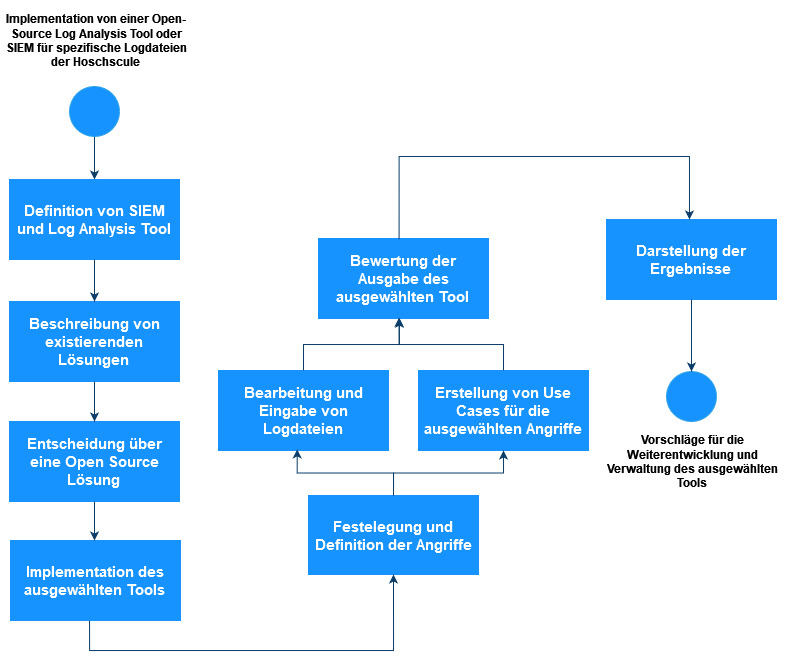
\includegraphics[width=1\textwidth]{assets/1_p1.jpg}
   \caption[Aufbau dieser wissenschaftlichen Recherche]
   {Aufbau dieser wissenschaftlichen Recherche \\Quelle: Eigene Darstellung }
   \centering
\end{figure}



